\section{Hybrid Job Placement}
\label{sec: hybrid placement}

Based on our experiments with two workloads, the ``bullying" is inevitable when the dragonfly network is configured with random placement and (progressive) adaptive routing. 
The precaution to stop the ``bullying" is to avoid network sharing between concurrently running jobs, 
and contiguous placement and minimal routing could be an effective way. 
However, the network would suffer severe local congestion and unbalanced utilization when contiguous placement and minimal routing is in use. 
Running each job with dedicated routing policy is unrealistic, 
since routing policy is part of system configuration which can not be changed on the fly upon job submission. 
Assigning preferable allocation to each job based on its communication intensity is applicable for the batch scheduler with intelligent job placement policy. 



We propose a hybrid job placement policy to assign each job with preferable allocation. 
According to the hybrid placement policy, 
the less communication-intensive jobs get contiguous allocation to partially avoid network sharing with the ``bully", 
while the communication-intensive jobs get random allocation in order to share network resource with each other. 
When Workload~\Rmnum{1} is running on the dragonfly network with hybrid placement policy, 
AMG gets contiguous allocation, MultiGrid and CrystalRouter get random allocations. 
The experiment results show that hybrid placement performs comparably as random placement for improving network performance and mitigates the degradation of AMG caused by the ``bullying".
\footnote{The analysis about network traffic and saturated time are omitted in this section due to page limit.}


%\subsection{Network Performance Analysis}
%
%Hybrid placement is also coupled with three routing policies, minimal, adaptive and progressive adaptive, denoted respectively as HM, HA and HPA. As presented in section~\ref{sec: workload-1 network analysis} and~\ref{sec: workload-2 network analysis}, random placement outperforms contiguous placement in terms of network performance, the analysis in this section only focuses on the comparison between hybrid and random placement policies. 
%
%\begin{table}[ht]
%\begin{center}
%\caption{Average time spent on communication by all MPI ranks when Workload I is running on dragonfly network under hybrid placement and random placement policies.} 
%\label{tab: hyb-placement-wkld-commtime}
%\begin{tabular}{l c c c c c c }
%\toprule % Top horizontal line
%\toprule
%&\multicolumn{6}{c}{Placement and Routing Configurations} \\
%\cmidrule(l){2-7}
%          & HM & HA & HPA & RM & RA & RPA \\ % Column names row
%\midrule % In-table horizontal line
%Time(ms)  &273 &255 &255 &255 &265 &264  \\ % Content row 1
%%\midrule
%%Workload II &1747 &1991 &1991 &1791 &2367 &1965 \\
%\midrule % In-table horizontal line
%\bottomrule % Bottom horizontal line
%\end{tabular}
%\end{center}
%\end{table}
%
%Due to page limit, we only present the average communication time spent by Workload~\Rmnum{1} for the evaluation of the network performance.
%\footnote{The analysis about network traffic and saturated time are omitted in this section due to page limit.}
%As shown in Table~\ref{tab: hyb-placement-wkld-commtime}, 
%hybrid placement coupled with (progressive) adaptive routing (HA, HPA) can guarantee the same performance as random placement coupled with minimal routing (RM), thus the average workload communication time stays unchanged. 
%When hybrid placement coupled with minimal routing (HM) is in use, 
%the network performance declines  as indicated by the increasing average communication time. 
%The consecutive groups assigned to AMG results in the diminishing of network resource shared by MultiGrid and CrystalRouter, 
%causing unbalanced utilization over the network.  



%\subsection{Individual Application Analysis}

\begin{figure*}[t!]
    \centering
    \begin{subfigure}[t]{0.32\textwidth}
        \centering
        \includegraphics[height=1.3 in]{hyb-plcmt/mg/commtime}
        \caption{MultiGrid Communication Time}
        \label{fig:hyb-plcmt-mg-commtime}
    \end{subfigure}\hfill
    \begin{subfigure}[t]{0.32\textwidth}
        \centering
        \includegraphics[height=1.3 in]{hyb-plcmt/cr/commtime}
        \caption{CrystalRouter Communication Time}
        \label{fig:hyb-plcmt-cr-commtime}
    \end{subfigure}\hfill
    \begin{subfigure}[t]{0.32\textwidth}
        \centering
        \includegraphics[height=1.3 in]{hyb-plcmt/amg/commtime}
        \caption{AMG Communication Time}
        \label{fig:hyb-plcmt-amg-commtime}
    \end{subfigure}
   \caption{Application communication time. Workload~\Rmnum{1} is running with all placement and routing configurations.}
   \label{fig:hyb-plcmt-apps-commtime}
\end{figure*}

The communication time of each application under all placement and routing configurations are presented in Figure~\ref{fig:hyb-plcmt-apps-commtime}. 
As shown in Figure~\ref{fig:hyb-plcmt-mg-commtime} and~{fig:hyb-plcmt-cr-commtime},
MultiGrid and CrystalRouter have similar performance with hybrid placement (HM, HA, HPA) as compared with random placement (RM, RA, RPA),
since they are still assigned with random allocations in the hybrid placement policy. 
The performance of AMG is significantly improved when hybrid placement configurations are in use. 
The communication time of AMG are reduced by half when the placement policy switched from random to hybrid, 
as shown in Figure \ref{fig:hyb-plcmt-amg-commtime}. 
This is due the contiguous allocation assigned to AMG in the hybrid placement policy. 
When being coupled with minimal routing, hybrid placement and contiguous placement have similar performance for AMG. 
However, when (progressive) adaptive routing are in use, the traffic from MultiGrid and CrystalRouter still might be redirected to the routers serving AMG. 
Since AMG is less communication-intensive and can not fully utilize network, 
it is likely that the intermediate routers picked for the traffic from MultiGrid and CrystalRouter could be from AMG's groups. Both the communication-intensive and the less intensive application can benefit from hybrid placement coupled with (progressive) adaptive routing.


The experiments with hybrid placement demonstrate that assigning each application with its preferable allocation can mitigate the negative effect of the ``bullying", in the meanwhile, 
the network can still reach the optimal performance.
Compared with random placement policy, hybrid placement can guarantee comparable network performance, by enabling network sharing between communication intensive applications .
It can also mitigate the performance degradation of less communication-intensive applications, 
by assigning them with contiguous allocation to partially avoid network sharing.
Unlike random placement indulging the ``bullying", hybrid placement can restrain it to some extent.
Hybrid placement policy is worthy of consideration for the adoption on dragonfly systems in the future.


